% normaliser les images par m sig de image net 
% 3. 
\chapter{Transfer Learning}
\graphicspath{{figs/2a/}}

The exploration focuses on Transfer Learning, where we adapt a well-known deep learning model -- VGG16 -- for new applications. This process involves utilizing the VGG16 architecture, originally designed for extensive image recognition, to comprehend and perform image classification on the 15 Scene dataset. It highlights how transfer learning makes existing models adaptable to new tasks and showcases their flexibility in addressing diverse real-world image processing challenges.

\section{VGG16 Architecture}

Examining the depths of neural network structures reveals the strong capabilities of models such as VGG16. Initially created for extensive image recognition, VGG16's complex layers of convolution and pooling highlight the advancements in deep learning. In this section, we explore the architecture of VGG16, breaking down its layers and understanding how they work together to extract features and classify images. This investigation not only clarifies the model's design but also sets the foundation for its practical use in various image processing tasks.

\paragraph{1. $\bigstar$ Knowing that the fully-connected layers account for the majority of the parameters in a model, give an estimate on the number of parameters of VGG16.}

There are three fully-connected layers at the end of the VGG16 architecture. Calculating their weights is relatively straightforward. We take into account the inclusion of biases.

\begin{itemize}
    \item The first fully-connected layer receives an input of size 7 by 7 by 512 (the resulting output of the convolutional layers), which equals an input size of 25,088. Knowing that there are 4,096 neurons, this layer has a total of $(25,088 + 1) \times 4,096 = 102,764,544$ trainable weights.
    \item The second fully-connected layer receives the input from the previous layer, which is 4,096, and also consists of 4,096 neurons, resulting in $(4,096 + 1) \times 4,096 = 16,781,312$ trainable weights.
    \item Lastly, the third fully-connected layer, consisting of 1,000 neurons, has $(4,096 + 1) \times 1,000 = 4,097,000$ trainable weights.
\end{itemize}

Thus, the fully connected layers account for a total of 123,642,856 parameters. We can confidently state that they represent at least 85\% of the model, implying there should be around \textbf{140 million parameters} to learn. If we consider a margin of 5\%, there should be between 137,380,951 and 154,553,570 parameters.

We can readily confirm that the convolutional layers account for 14,714,688 parameters, meaning that there are actually 138,357,544 parameters in VGG16, meaning the fully-connected layers accounts to 89\% of parameters.

% conv1 - 2 layers
% ((3*3*3)+1)*64 = 1,792
% ((64*3*3)+1)*64 = 36,928
% TOTAL 38720

% conv2 - 2 layers
% ((64*3*3)+1)*128 = 73,856
% ((128*3*3)+1)*128 = 147,584
% TOTAL 221440

% conv3 - 3 layers
% ((128*3*3)+1)*256 = 295,168
% ((256*3*3)+1)*256 = 590,080
% ((256*3*3)+1)*256 = 590,080
% TOTAL 1475328

% conv4 - 3 layers
% ((256*3*3)+1)*512 = 1,180,160
% ((512*3*3)+1)*512 = 2,359,808
% ((512*3*3)+1)*512 = 2,359,808
% TOTAL 5,899,776. 

% conv5 - 3 layers
% ((512*3*3)+1)*512 = 2,359,808
% ((512*3*3)+1)*512 = 2,359,808
% ((512*3*3)+1)*512 = 2,359,808
% TOTAL 7,079,424
% TOTAL CONVS = 14,714,688

% fc1
% (7x7x512 + 1)*4096 = 102,764,544

% fc2
% (4096+1)*4096 = 16,781,312

% fc3
% (4096+1)*1000 = 4,097,000
% TOTAL FC - 123,642,856
% TOTAL VG16 - 138,357,544

\paragraph{2. $\bigstar$ What is the output size of the last layer of VGG16? What does it correspond to?}
The output size of the last layer of VGG16 is 1000. It corresponds to the 1000 classes of the ImageNet dataset that the model has been trained on. Each element in this output vector represents  the network's prediction scores for a specific class in the ImageNet dataset, and the class with the highest score is considered the predicted class for our given input image.

\paragraph{3. \textbf{Bonus}: Apply the network on several images of your choice and comment on the results.}

In \Cref{fig:vgg16}, we present the results of our network's application to six diverse images, encompassing different scenarios. These include two common images featuring a tuxedo cat and a Shih Tzu dog, along with two whimsical images and two images of Komondor dogs. The whimsical images consist of a close-up of a wombat and a photomontage featuring a dog. The Komondor images, in particular, provide an interesting challenge; one is clearly a dog, while the other's unique coat might humorously resemble a mop.

The network's predictions showcase its ability to recognize certain animal features, yet they also highlight its limitations in classification. It correctly identifies the wombat, cardigan dog, and Komondor without confusing the latter with a mop. However, it misclassifies the Shih Tzu as a Miniature Poodle, with a Lakeland Terrier as a close second, indicating confusion between breeds with similar appearances. The tuxedo cat is inaccurately labeled as an Egyptian Mau, emphasizing the network's difficulty in precise breed identification—a challenge partly attributed to the absence of highly specific categories within ImageNet's 1000 classes. Nevertheless, the tuxedo cat is still classified as a cat. These outcomes not only identify areas for improvement in the network's classification capabilities but also suggest the potential benefits of transfer learning. The identified errors offer valuable insights for further refining the model.

% \begin{figure}[H]
%     \centering
%     \includegraphics*[width=0.95\textwidth]{predictions.pdf}
%     \caption{Prediction of VGG16 on few images}
%     \label{fig:vgg16}
% \end{figure} % BOBR!!!!!!

\begin{figure}[H]
    \centering
    \begin{subfigure}{0.95\textwidth}
        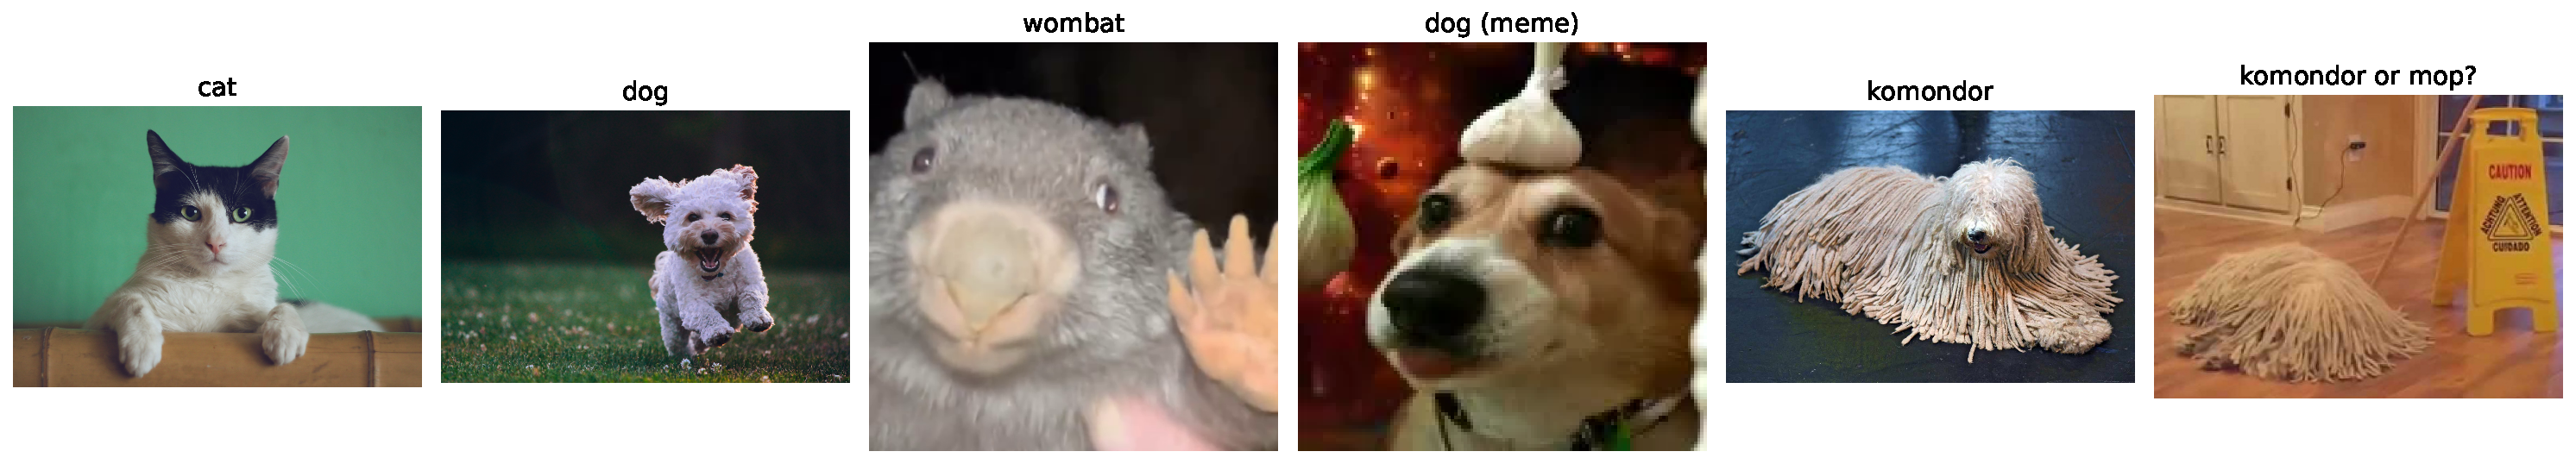
\includegraphics[width=\textwidth]{original_images}
        \caption{}
        \label{subfig:original_images}
    \end{subfigure}
    \begin{subfigure}{0.95\textwidth}
        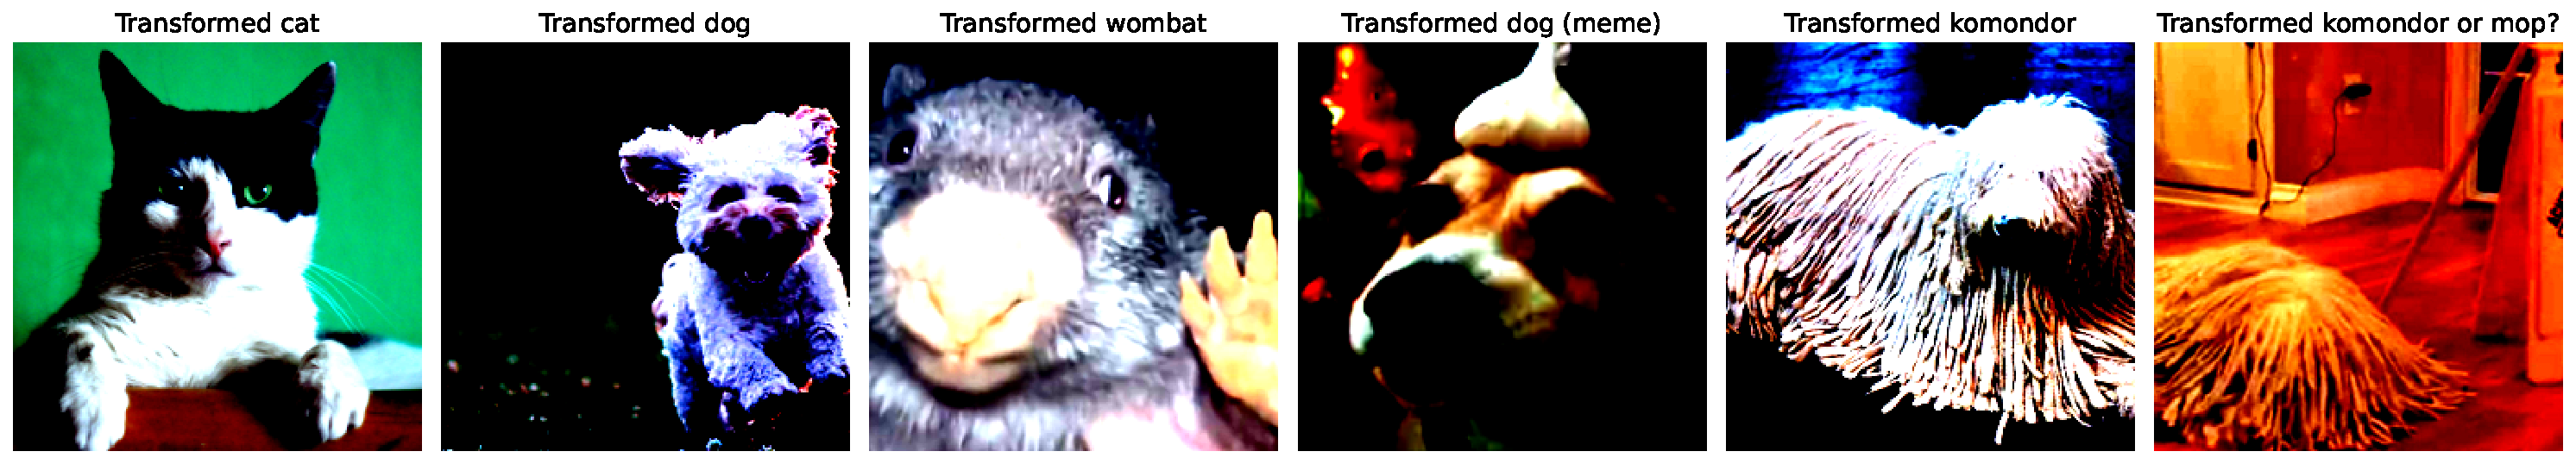
\includegraphics[width=\textwidth]{transformed_images}
        \caption{}
        \label{subfig:transformed_images}
    \end{subfigure}
    \begin{subfigure}{0.95\textwidth}
        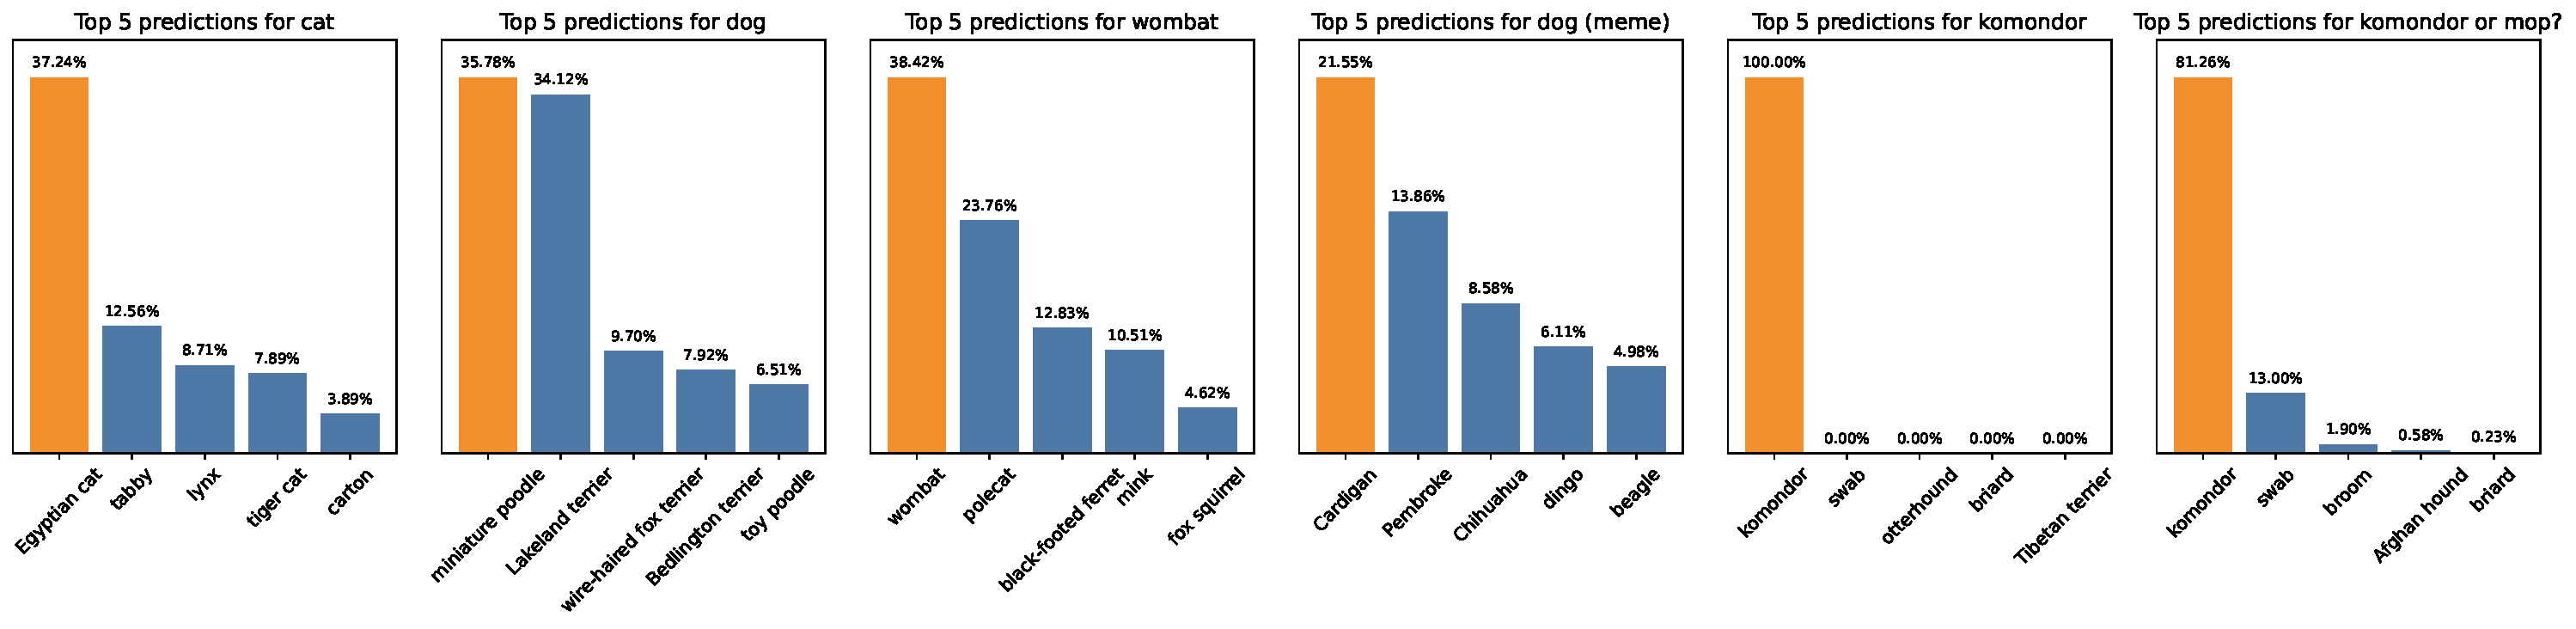
\includegraphics[width=\textwidth]{prediction_plots}
        \caption{}
        \label{subfig:prediction_plots}
    \end{subfigure}
    \caption{Performance evaluation of VGG16 pre-trained on ImageNet: (a) Original images, (b) Transformed images normalized and resized to $224 \times 224$, and (c) Top 5 predicted classes}
    \label{fig:vgg16}
\end{figure}


\paragraph{4. \textbf{Bonus}: Visualize several activation maps obtained after the first convolutional layer. How can we interpret them?}
Let $A_{ij}$ denote the activation map located at the $i$th row and $j$th column, where $i$ and $j$ are both in the range of $[1, 8]$.

In \Cref{fig:activation_cat}, we showcase the 64 feature maps obtained after applying the first convolutional layer of VGG16 to the tuxedo cat image. Furthermore, we include activation maps for the five preceding images in Appendix \Cref{appendix:activation_maps}.

Each activation map corresponds to a unique filter applied to the original image, capturing a diverse array of features. Some maps highlight edges or textures (e.g., $A_{12}$, $A_{13}$, $A_{88}$), while others respond to background elements (e.g., $A_{26}$, $A_{28}$), color contrasts (e.g., $A_{41}$, $A_{62}$), or specific shapes (e.g., $A_{33}$, $A_{65}$) within the image. It is important to note that these initial layers are primarily designed to detect low-level features, which become progressively more abstract and complex in deeper layers. Additionally, these maps consistently serve specific purposes regardless of the input image, indicating a dedicated function for each activation map. Thus, our interpretation stays true for the images in Appendix \Cref{appendix:activation_maps}.

\begin{figure}[H]
    \centering
    \includegraphics*[width=0.95\textwidth]{activation_cat}
    \caption{Activation maps obtained after the first convolutional layer of VGG16, on the tuxedo cat image}
    \label{fig:activation_cat}
\end{figure}

\section{Transfer Learning with VGG16 on 15 Scene}

The concept of transfer learning plays a significant role when it comes to applying pre-trained models to unfamiliar fields. In this section, our focus will be on how VGG16 can be cleverly repurposed for different yet related tasks. This approach highlights the adaptability of deep learning models and emphasizes the idea that existing knowledge encoded within a trained network can be successfully applied to new areas, a fundamental principle in modern machine learning research.

\subsection{Approach}
\paragraph{5. $\bigstar$ Why not directly train VGG16 on 15 Scene?}
The 15 Scene dataset is quite small compared to the massive ImageNet dataset that VGG16 was originally trained on. VGG16 requires a lot of data to generalize well and to avoid overfitting. Moreover, training such a model from scratch is computationally expensive and time-consuming.

\paragraph{6. $\bigstar$ How can pre-training on ImageNet help classification for 15 Scene?}
ImageNet is a vast and diverse dataset, containing millions of images distributed across numerous categories. A model pre-trained on this dataset acquires a broad spectrum of features, ranging from basic edge and texture detection to intricate patterns. These acquired features provide a robust initial foundation for extracting meaningful information from the 15 Scene images, even when the particular scenes or objects present in the 15 Scene dataset differ from those in ImageNet. This approach offers several advantages, especially considering the relatively small size of our dataset. It helps address issues related to insufficient training data, such as overfitting. Additionally, it speeds up the training process because the model only needs fine-tuning of the previously learned features to adapt to the specific characteristics of the new dataset, eliminating the need to start the learning process from scratch.

\paragraph{7. What limits can you see with feature extraction?}
The effectiveness of transferred features depends on the similarity between the source task, for which the model was originally trained, and the target task. When the target task significantly differs from the source task, the extracted features may not be relevant or useful, and they may fail to capture the nuanced details required for achieving high accuracy. For instance, using a model trained on natural images for tasks like medical images or satellite imagery might not produce optimal results. To adapt such models to new domains, additional fine-tuning or even complete retraining with domain-specific data is often necessary, which can consume significant computational resources.

It's important to note that biases present in the pre-training dataset can influence the features extracted by the model. If the pre-training data is not representative or contains inherent biases, these biases can unintentionally affect the performance on the target task. Moreover, the utilization of models like VGG16 demands substantial computational resources, including both memory and processing power, which can present limitations, especially in resource-constrained environments.

\subsection{Feature Extraction with VGG16}
\paragraph{8. What is the impact of the layer at which the features are extracted?}
In CNNs, earlier layers typically capture fundamental features such as edges and textures, while deeper layers capture increasingly complex and high-level features that are more abstract and representative of the specific content within an image.

For some tasks, the simpler features extracted from the early layers may suffice, while for more intricate tasks (such as distinguishing between very similar categories), the deeper features can be more valuable. Early layers are generally more adaptable across various image types and tasks, whereas deeper layers tend to be more specialized and specific to the types of images and tasks the network was initially trained on.

\paragraph{9. The images from 15 Scene are black and white, but VGG16 requires RGB images. How can we get around this problem?}
Image from 15 scene are black and white so they only have one channel. VGG requires 3 channel RGB images. The easiest workaround is to replicate the single channel of the grayscale image across the three RGB channels. Another solution is to average the weights of the first convolutional layer (which is responsible for the RGB channels) so that it can directly accept grayscale images.

\subsection{Training SVM classifiers}
\paragraph{10. Rather than training an independent classifier, is it possible to just use the neural network? Explain.}
Absolutely, it is possible to use the neural network itself instead of training an independent classifier. In the case of models like VGG16, the final classification layer is essentially a neural network. If the classification task is similar to what VGG16 was originally trained for, we can fine-tune this neural network for our specific task. However, if the task is substantially different from the original one, it may not be ideal to retain the pre-trained classifier, as it might not perform well on new classes.

The decision between using the pre-trained neural network or training an independent classifier, such as an SVM, depends on the nature of the task and the available data. Using the pre-trained network can save time and computational resources, but fine-tuning or retraining may be necessary for optimal results on different tasks. Using a simpler classifier like an SVM can be a good compromise, leveraging the deep features extracted by the neural network while providing a more interpretable decision boundary.

\subsection{Going further}
\paragraph*{11. For every improvement that you test, explain your reasoning and comment on the obtained results.}

In the study of transfer learning from VGG16 pretrained on ImageNet for Scene15 classification, the depth of the feature extraction layer emerged as a significant factor. Extracting features after the first fully connected layer (ReLU6) versus the second (ReLU7) offers the same dimensionality (4096 features), yet stopping after the first yields better results. Results are displayed on \Cref{tab:depth_influence}. This suggests that the initial fully connected layers may capture more generalizable features beneficial for the task at hand. Using all three fully connected layers (up to ReLU8) reduces feature dimensionality to 1000 and leads to poorer performance, likely due to over-specialization to ImageNet.

\begin{table}[H]
    \centering
    \begin{tabular}{@{}cccc@{}}
        \toprule
        \textbf{Layer Extracted} & \textbf{Feature Dimensionality} & \textbf{Accuracy (Non-Normalized)} & \textbf{Accuracy (Normalized)} \\
        \midrule \midrule
        ReLU6                    & 4096                            & \textbf{0.906}                     & \textbf{0.912}                 \\
        ReLU7                    & 4096                            & 0.896                              & 0.896                          \\
        ReLU8                    & 1000                            & 0.861                              & 0.880                          \\
        \bottomrule
    \end{tabular}
    \caption{Performance comparison based on the depth of feature extraction in VGG16, indicating accuracy for features extracted at ReLU6, ReLU7, and ReLU8 using an SVM with $C$ = 1, and whether or not the data were normalized.}
    \label{tab:depth_influence}
\end{table}

Additionally, the choice of feature extraction layer, whether it be the first fully-connected layer, second, or third, did not have a discernible impact on the time required for feature extraction or the time taken to train a SVM. We conducted a grid search over 5-fold cross-validation to fine-tune the SVM parameters and present the results in \Cref{tab:svm_tuned}. The variation in the optimal $C$ values across different layers (ReLU6, ReLU7, ReLU8) sheds light on key aspects of feature complexity and generalizability. Higher $C$ values suggest the need for stronger regularization, possibly due to the features being more intricate and specialized towards the ImageNet dataset, hence less adaptable to the Scene15 dataset.

\begin{table}[H]
    \centering
    \begin{tabular}{@{}cccc@{}}
        \toprule
        \textbf{Layer Extracted} & \textbf{Best $C$ value} & \textbf{Cross-validation score} & \textbf{Accuracy} \\
        \midrule \midrule
        ReLU6                    & 10                     & \textbf{0.920}                  & \textbf{0.910}    \\
        ReLU7                    & 100                     & 0.905                           & 0.899             \\
        ReLU8                    & 5                       & 0.894                           & 0.888             \\
        \bottomrule
    \end{tabular}
    \caption{Tuning results for SVM using features extracted from different layers of VGG16, highlighting the best $C$ value, cross-validation score, and accuracy, using normalized data.}
    \label{tab:svm_tuned}
\end{table}

We also explored the effectiveness of employing a custom Multi-Layer Perceptron (MLP) as an alternative to using a SVM for classification. The architecture of our MLP is outlined in Table \ref{tab:mlp_architecture}. The motivation behind this approach was to examine whether a neural network, capable of end-to-end learning, could outperform the conventional method of SVM classification when working with features extracted from VGG16. This experiment was carried out in two variations: one where the MLP served as a standalone classifier for the extracted features, and another where the MLP was integrated into a modified VGG16, functioning as the final layers, with the flexibility of either freezing or fine-tuning the earlier layers.

The experiment yielded two key outcomes: the standalone MLP achieved an accuracy of 0.8958, while the MLP integrated into VGG16 achieved an accuracy of 0.8938, both after 20 epochs. These results, though slightly lower than those obtained with an SVM, suggest that the more complex end-to-end learning approach of a neural network does not necessarily lead to superior performance compared to using a simpler model like SVM on pre-extracted features. This observation reinforces the notion that in certain transfer learning scenarios, particularly when the extracted features are already robust, simpler models can be equally, if not more, effective than their more complex counterparts, while being much more computationally efficient.

\begin{table}[H]
    \centering
    \begin{tabular}{@{}lll@{}}
        \toprule
        \textbf{Layer Type}                           & \textbf{Output Size} & \textbf{Parameters}                   \\ \midrule
        Linear                                        & 1024                 & 4096 $\times$ 1024 + 1024 = 4,195,328 \\
        ReLU                                          & -                    & -                                     \\
        Dropout                                       & -                    & rate = 0.2                            \\
        Linear                                        & 512                  & 1024 $\times$ 512 + 512 = 524,800     \\
        ReLU                                          & -                    & -                                     \\
        Dropout                                       & -                    & rate = 0.2                            \\
        Linear                                        & 15                   & 512 $\times$ 15 + 15 = 7695           \\
        \midrule
        \multicolumn{2}{l}{\textbf{Total parameters}} & 4,727,823                                                    \\
        \bottomrule
    \end{tabular}
    \caption{Architecture of the Multi-Layer Perceptron (MLP) used in the VGG16 modification.}
    \label{tab:mlp_architecture}
\end{table}

Lastly, we explored alternative architectures for transfer learning, extending our considerations beyond VGG16 to leverage the advancements made in pre-trained networks since 2014. Our focus shifted to attention-based models, particularly Vision Transformers, renowned for their superior performance on ImageNet. In our experiments, we chose the \texttt{vit\_b\_16} model, celebrated for its efficient parameter utilization (with 37.43\% fewer parameters compared to VGG16) and improved accuracy (a 9.48\% boost in top-1 accuracy compared to VGG16).  In our initial analysis, we evaluated the performance of this model using the first six images and observed a noticeable increase in the model's assertiveness in its predictions. For instance, the model exhibited significantly higher confidence in correctly identifying a wombat as a wombat, with a confidence level of 97.48\% for the fine-tuned weights compared to 38.42\% in VGG16. Results are available in Appendix \Cref{appendix:vit}, presented in \Cref{fig:vit_scratch} and \Cref{fig:vit_refined}.


Feature extraction occurred after the encoder, specifically at the linear layer of the classifier. Notably, we evaluated weights refined via end-to-end fine-tuning (IMAGENET1K\_SWAG\_E2E\_V1) against those trained from scratch (IMAGENET1K\_V1). Our findings are presented in \Cref{tab:vit_transferlearning} and \Cref{tab:vit_svm_tuned}. It's worth noting that tuning the SVM with Vision Transformer features led to superior results when compared to the tuned SVM trained using VGG16 features, resulting in a significant 2.1\% increase in accuracy. As expected, the utilization of IMAGENET1K\_SWAG\_E2E\_V1 weights naturally provided the best performance, owing to their superior performance on ImageNet-1K. Additionally, it's important to mention that the feature extraction process for Vision Transformers did indeed take a bit longer. Specifically, Vision Transformers processed at a rate ranging from 6 to 12 batches per second, while VGG ranged from 15 to 20 batches per second.

\begin{table}[H]
    \centering
    \begin{tabular}{@{}cccc@{}}
        \toprule
        \textbf{Weights}  & \textbf{Accuracy (Non-Normalized)} & \textbf{Accuracy (Normalized)} \\
        \midrule \midrule
        IMAGENET1K\_V1            & 0.911                              & 0.918             \\
        IMAGENET1K\_SWAG\_E2E\_V1 & \textbf{0.917}                     & \textbf{0.925}    \\
        \bottomrule
    \end{tabular}
    \caption{Performance comparison based on the weights used for Vision Transformer, using an SVM with $C$~=~1, and whether or not the data were normalized.}
    \label{tab:vit_transferlearning}
\end{table}

\begin{table}[H]
    \centering
    \begin{tabular}{@{}cccc@{}}
        \toprule
        \textbf{Weights} & \textbf{Best $C$ value} & \textbf{Cross-validation score} & \textbf{Accuracy (Normalized)} \\
        \midrule \midrule
        IMAGENET1K\_V1           & 1                       & 0.921                           & 0.918             \\
        IMAGENET1K\_SWAG\_E2E\_V1  & 5                       & \textbf{0.944}                  & \textbf{0.931}    \\
        \bottomrule
    \end{tabular}
    \caption{Tuning results for SVM using different sets of weights for Vision Transformer, highlighting the best $C$ value, cross-validation score, and accuracy, using normalized data.}
    \label{tab:vit_svm_tuned}
\end{table}